\documentclass[12pt]{beamer}
\usetheme{Hannover}
\usepackage{graphicx}
\usepackage{booktabs}
\usepackage[english]{babel}
\usepackage{kotex}
%\usepackage[pdfencoding=auto]{hyperref}
\hypersetup{pdfencoding=auto}
\usepackage{ulem}
\usepackage[per-mode=symbol]{siunitx}
\sisetup{inter-unit-product =$\cdot$}
\usepackage{color}
\usepackage{ulem}
\usepackage{amsmath,amssymb}
\graphicspath{{images/}}
\title[\LaTeX - Day 1]{\LaTeX 입문 - Day 1}

\author{14041 박승원}
\institute[GSHS]
{과학영재학교 경기과학고등학교 \TeX 사용자협회 \\ 
	\medskip
	psw14041@gmail.com (@seungwonpark GitHub)
}
\date{마지막 수정일 : \today}


\AtBeginSection[]{
	\begin{frame}
		\vfill
		\centering
		\begin{beamercolorbox}[sep=8pt,center,shadow=true,rounded=true]{title}
			\usebeamerfont{title}\insertsectionhead\par%
		\end{beamercolorbox}
		\vfill
	\end{frame}
}

\begin{document}

\begin{frame}
\titlepage % Print the title page as the first slide
\end{frame}

\section{\LaTeX}
\begin{frame}{\LaTeX 이란?(Day 0와 동일)}
	\begin{itemize}
		\item 개발
		\begin{itemize}
			\item Donald Knuth 에 의해 \TeX 개발됨(1978)
			\item \TeX 을 쉽게 사용하기 위한 매크로 : \LaTeX
			\item 발음 : [텍], [레이텍]
		\end{itemize}
		\item 특징
		\begin{itemize}
			\item 수식입력 기능, 자동 ToC\footnote{Table of Contents}, LoF\footnote{List of Figures}, LoT\footnote{List of Tables} 생성
			\item 편리한 labeling 및 referencing
			\item 많은 학회에서 tex 으로 논문을 투고받음
			\item 초기 설정 이후 내용 작성에만 집중 가능
			\item 논문, 발표자료, 시험지, 악보 등등... 만능!
		\end{itemize}
	\end{itemize}
\end{frame}
\subsection{\TeX 시작하기}
\begin{frame}{\TeX 설치하기(Day 0와 동일)}
	KTUG(Korean \TeX User Group)\footnote{한글 \TeX 사용자 그룹, [케이턱]}
	\begin{itemize}
		\item \TeX 사용 환경 조성 : TeXLive
		\item 한글을 사용하기 위한 TeXLive 가 koTeXLive
		\item 내려받기 - 설치 방법대로 따라간다.
		\item 용량이 약 2GB. 시간적 여유를 가지고 설치.
	\end{itemize}
	\TeX 문서 편집기
	\begin{itemize}
		\item TeXLive에서 기본 제공 : TeXWorks / TeXshop
		\item 하지만 TeXStudio\footnote{texstudio.org}가 훠---얼씬 편하다!
	\end{itemize}
\end{frame}
\begin{frame}{GSHS TeX Society}
	경기과학고 TeX 사용자협회 Since 2015.
	\begin{itemize}
		\item \TeX 스터디(?)가 초기 목적 - gshslatexintro
		\item R\&E, 졸업논문 등의 tex, cls 파일을 수정 및 보완하는 \TeX 사용자 협회로 발전
	\end{itemize}
	\url{http://gshslatexintro.github.io} \footnote{현재 \url{chanspi.ddns.net/gshs/LaTeX}으로 리다이렉트됨.}
	\begin{itemize}
		\item 각종 양식 및 입문서, 예시 제공.
		\item \sout{곧 송죽학사에 관련 탭이 개설될 예정.}
	\end{itemize}
\end{frame}
\begin{frame}{GSHS TeX Society}
	\framesubtitle{Flowchart}
	\begin{figure}[h]
		\centering
		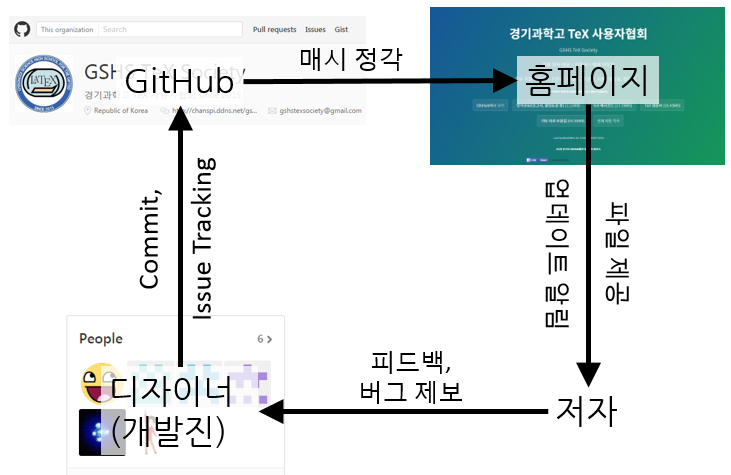
\includegraphics[width=\textwidth]{gshstexsociety.png}
	\end{figure}
\end{frame}
\subsection{\TeX 문서 구조}
\begin{frame}{\TeX 문서 구조}
	Preamble[프림블]
	\begin{itemize}
		\item 쉽게 말하자면 문서의 header.
		\item 문서의 유형(documentclass)\footnote{문서 유형의 종류에 관해서는 부록을 참조 바람}, package 들을 선언
		\item 外 필요한 환경설정 및 명령어 선언
	\end{itemize}
	Body(본문)
	\begin{itemize}
		\item 위키백과 문서 편집과 비슷?
		\item 아래아한글, MS Word 는 WYSIWYG...
	\end{itemize}
\end{frame}
\begin{frame}{Preamble}
	예시 : 이 문서의 Preamble. 
	\begin{figure}
		\centering
		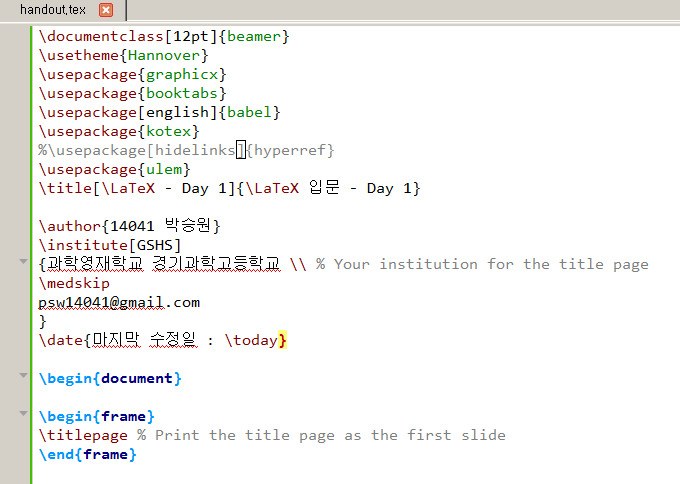
\includegraphics[width=.9\textwidth]{texception.png}
	\end{figure}
\end{frame}
\begin{frame}{본문 : WYSIWYG / \LaTeX}
	\begin{figure}
		\centering
		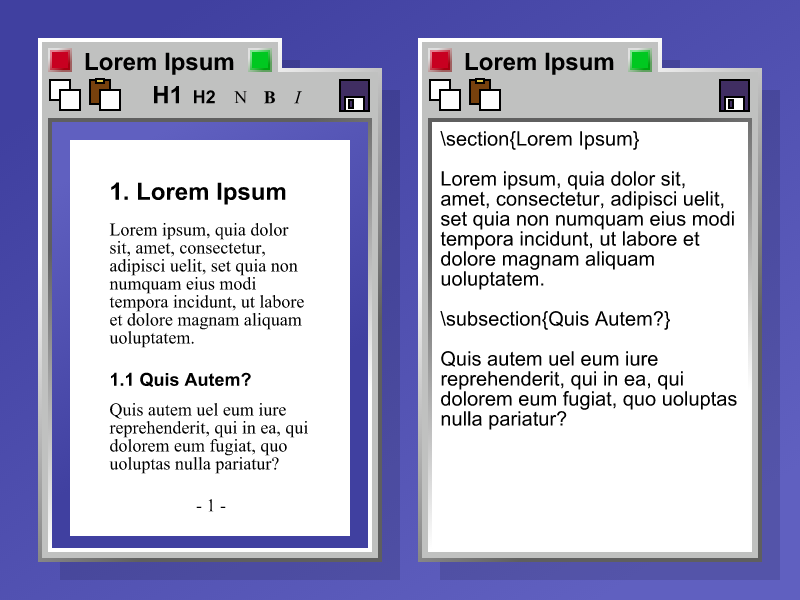
\includegraphics[width=.9\textwidth]{wysiwyg.png}
	\end{figure}
	Illustration by Shinobu in Wikimedia
\end{frame}
\begin{frame}{Template 등록}
	매번 \TeX 문서를 작성하기 시작할 때마다 preamble 을 작성하는 것은 매우 번거로운 일이다. 
	
	경기과학고 \TeX 사용자협회에서 제작한 간단한 Template\footnote{\url{https://github.com/gshslatexintro/examples/raw/master/sample_document/sample_document.tex}} 을 내려받아 TeXstudio 에서 User template 으로 지정해 놓으면 편하다.
	\vspace{0.7cm}
	
	해당 파일을 연 상태에서 TeXstudio - File - Make Template
\end{frame}
\section{\TeX 과 친해지기}
\subsection{수식 입력}
\begin{frame}{`mathmode'}
	\begin{enumerate}
		\item \$ ... \$ : 수식 \\
		$e^{i\pi}+1=0$
		\item \$\$ ... \$\$ : 가운데 정렬된 수식
		$$e^{i\pi}+1=0$$
		\item \textbackslash begin\{equation\} ... \textbackslash end\{equation\} : 번호가 매겨진 수식\footnote{equation 환경 외에도 여럿 있음. 부록 참조 바람.}
		\begin{equation}
		e^{i\pi}+1=0
		\end{equation}
	\end{enumerate}
	수식에 붙은 번호를 referencing 할 수 있는데, 이건 다음 시간에...
\end{frame}
\begin{frame}{수식 문법}
	TeXStudio의 왼쪽 바에서 전부 찾아볼 수 있다.
	\begin{itemize}
		\item \textbackslash sin\{...\}, \textbackslash log\{...\} : 삼각함수, 로그함수는 기울여 쓰면 안되므로 이렇게 써야 한다.
		\item \textbackslash frac\{(num)\}\{(den)\} : 분자 num, 분모 den 인 분수
		\item \textbackslash sqrt [n]\{x\} : $x$의 $n$제곱근
		\item \textbackslash sum\_\{i=1\}\textasciicircum{n}\{...\} : 시그마 합 표기법.
		\item \textbackslash begin \{cases\} ... \textbackslash end\{cases\} : 중괄호로 경우 나누기
	\end{itemize}
	용례는 다음 페이지 참조. {\footnotesize (대괄호와 중괄호 구분에 유의!)}
\end{frame}
\begin{frame}{수식 용례}
	코드 : \footnote{\url{http://pastebin.com/Qt1MVcSb}}
	$$ \sin{\pi} = 0 $$
	$$ \log_{2}{8} = 3 $$
	$$ \frac{6}{3} = 2 $$
	$$ \sqrt[3]{8} = 2 $$
	$$ \sum_{i=1}^{n}{1} = n $$
	\begin{equation}
	f(n) = \begin{cases} 0 &\mbox{if } n<0 \\ 
	1 & \mbox{if } n\geq 1 \end{cases}
	\end{equation}
\end{frame}
\subsection{워드프로세서 기본사항}
\begin{frame}{특수문자}
	\TeX 에서 바로 사용할 수 없는 문자 : 
	\begin{center}
		\textbackslash, \#, \$, \%, \&, \{, \}, \_ \textasciitilde, \textasciicircum
	\end{center}
	다음과 같이, 대부분의 경우 단순히 backslash를 붙여주면 된다.
	\begin{center}
		\textbackslash textbackslash, \textbackslash\#, \textbackslash\$, \textbackslash\%, \textbackslash\&, \textbackslash\{, \textbackslash\}, \textbackslash \_ , \textbackslash textasciitilde, \textbackslash textasciicircum 
	\end{center}
	Tip : \% 는 코드의 주석 처리를 위해 사용된다. 여러 줄 주석처리는 여기\footnote{\url{http://tex.stackexchange.com/questions/17816/commenting-out-large-sections}} 를 참조
\end{frame}
\begin{frame}{띄어쓰기, 개행}
	\begin{itemize}
		\item \TeX 코드에서 띄어쓰기를 아무리 많이 해도 결과물에서는 띄어쓰기가 한번만 된다. \\
		`\textasciitilde' 를 사용하여 이~~~~렇게 띄울 수 있다.
		\item 보통 개행을 위해서는 \textbackslash\textbackslash 가 자주 이용된다. 단순히 2회 개행해 놓아도 된다.
		\item \TeX 코드에서 한번 개행한 것으로는 결과물에서는 개행되지 않는다. 2회 개행해야 한다. \\
		사실 이 덕분에 문장 수정하기가 훨씬 좋아진다. 
	\end{itemize}
	여백을 만들어야 할 경우 \textbackslash vfill, \textbackslash vspace\{2cm\} 등을 사용 가능.
	
\end{frame}
\begin{frame}{각주, 들여쓰기}
	각주는 단순히 \textbackslash \{...\} 와 같이 사용하면 된다. 단, 표에서 사용할 경우 문제가 발생할 수 있다.
	\vspace{1cm}
	
	(기본적으로 조정이 되지만, 처음에 익숙하지 않을 때는 단순히 \textbackslash indent, \textbackslash noindent 로 강제 조정할 수 있다.)
	
	2회 개행으로 개행했을 경우 들여쓰기가 되고, \textbackslash\textbackslash 로 개행했을 경우 들여쓰기가 없다. 
	
\end{frame}
\begin{frame}{좌측/우측/중앙 정렬}
	\begin{flushleft}
		좌측 정렬
	\end{flushleft}
	\begin{flushright}
		우측 정렬
	\end{flushright}
	\begin{center}
		중앙 정렬
	\end{center}
	각각 flushleft, flushright, center 환경을 사용하면 된다.
	
	예시 : \textbackslash begin\{center\} 텍스트	\textbackslash end\{center\}
\end{frame}
\begin{frame}{페이지 넘김 및 편집용지}
	
	페이지 넘김은 \textbackslash newpage 또는 \textbackslash clearpage 를 사용. 책을 만들 경우 \textbackslash cleardoublepage
	\vspace{0.7cm}
	
	편집용지는 geometry 패키지를 참조하라. 
	
	\textbackslash usepackage[left=25mm,right=25mm,top=30mm,
	
	bottom=30mm]\{geometry\}
\end{frame}
\begin{frame}{글꼴 조정}
	\begin{itemize}
		\item \textbf{굵게} : \textbackslash textbf\{...\}
		\item \textit{이태릭} : \textbackslash textit\{...\}
		\item \textsf{산세리프}\footnote{본 문서는 beamer class 를 사용하기 때문에 기본 폰트가 산세리프이다. 한글의 경우 나눔고딕.} : \textbackslash textsf\{...\}
		\item {\color{blue} 색상} : color package 를 사용, \{ \textbackslash color \{blue\} ... \}
	\end{itemize}
	kotexlive 2013 기준으로, \TeX 의 기본 한글글꼴은 네이버에서 배포한 나눔명조 및 나눔고딕이다. 영어 기본 글꼴은 `Computer Modern' 이고, 필요할 경우 해당 package 를 사용하여 Times New Roman 을 사용할 수 있다. 사용방법 : \footnote{\url{http://pastebin.com/fZphiXGT}}
\end{frame}
\subsection{열거 환경}
\begin{frame}{열거 환경 : itemize / enumerate}
	용례 및 코드 : \footnote{\url{http://pastebin.com/Q9StmCgJ}}
	\begin{itemize}
		\item 본관에서는 주로 국어, 수학, 영어 과목을 수강한다.
		\item SRC에서는 물리를 비롯한 과학 과목들을 수강한다.
		\item 기숙사에서는 잠을 잘 수 있다.
	\end{itemize}
	\begin{enumerate}
		\item 측정을 개시한다.
		\item 일정한 전압을 가하고 온도가 평형상태에 도달할 때까지 기다린다.
		\item 전원 공급을 끊고, 측정을 종료한다.
	\end{enumerate}
\end{frame}
\section{부록}
\subsection{여러 수식 환경들}
\begin{frame}{equation / equation*}
	equation 환경을 쓰되, 번호를 매기고 싶지 않을 경우 사용한다. 
	이 방법 외에도, 그냥 \$\$ ... \$\$ 를 사용하거나,
	등식 맨 뒤에 \textbackslash notag 를 붙여도 된다. 코드 : \footnote{\url{http://pastebin.com/vsxT1MrY}}
	\begin{equation*}
		\mathcal{L} \equiv T-V
	\end{equation*}
	통상적으로 \TeX 에서는 equation* 외에도 *를 붙이면 번호가 매겨지지 않는다. 뒤에 설명할 align, gather 등도 align*, gather* 환경이 존재하며, section 과 같은 것도 section* 가 존재.
\end{frame}
\begin{frame}{검색하면 다 나온다!}
	\begin{itemize}
		\item align, aligned, gather, ... 다양한 수식 환경
		\item 괄호 크기 자동조정 : \textbackslash left( ... \textbackslash right)
		\item 수식의 태그 임의로 변경하기 : \textbackslash tag\{...\}
	\end{itemize}
	Tip : 품위있는(?) 논문에서는, 중요한 수식들은 모두 온점(.) 으로 마무리한다.
\end{frame}
\subsection{문서의 유형}
\begin{frame}{자주 사용되는 문서 종류}
	\begin{tabular}{|c|c|}
		\hline
		class & 설명 \\
		\hline
		\hline
		article & 단순 문서 \\
		\hline
		report & 보고서 및 논문 \\
		\hline
		book & 책 \\
		\hline
		beamer & 발표용 자료 제작 (이 문서에서도 사용됨) \\
		\hline
		sciposter & 포스터 제작 \\
		\hline
		letter & 편지 작성 \\ 
		\hline
	\end{tabular}
	\begin{itemize}
		\item 일단 우리가 보기에는 article 과 report 는 큰 차이는 없다.
		\item book 과 beamer 의 인상적인(?) 용례가 경기과학고 \TeX 사용자협회에 있으니 구경삼아 읽어본다면 재미있을 것이다.
	\end{itemize}
\end{frame}
\subsection{글꼴 조정}
\begin{frame}{글꼴 조정에 관하여}
	보통 사용되는 pdf\LaTeX 이 아닌 Xe\LaTeX 을 사용하여 \TeX 에서 `바탕' 이나 `굴림'을 사용할 수 있다. 용례는 경기과학고 \TeX 사용자협회의 `독서 독후감 양식' \footnote{\url{https://github.com/gshslatexintro/gshslatexintro/tree/master/gshs_reading}} 이 있다. 
	\vspace{1cm}
	
	다른 글꼴들을 사용하는 것도 불가능하지는 않으나 권장되지 않는다. \TeX 은 논문 작성에 특화된 학술 언어이다. 논문에서 여러 글꼴을 사용하는 것은 좋지 않다.
\end{frame}
\begin{frame}{한글 글꼴...}
	``사실 공식적인 양식이 hwp 나 word일 경우 발생하는 가장 큰 문제점은 (한글)폰트입니다. 영어의 경우 Times New Roman 을 쉽게 사용 가능하고, 한글의 경우 xetex을 이용하면 바탕, 굴림, 궁서를 넣을 수 있으나 신명조 같은거는 저작권법상 아래아한글 내에서의 사용만이 허락된 거라... (ttf파일을 가지고 있다면 텍 전용 폰트 파일인 tfm을 만드는 것은 크게 어렵지는 않습니다)  Arial 같은 영어폰트는 금방 하는데 한글 폰트는 KTUG에서 시키는 대로 해야돼요 ''
	
	$ \rightarrow $ 과학전람회와 같이 hwp 로 양식을 제공하는 경우 어쩔 수 없이 아래아한글로 작성해야 한다...
\end{frame}
\subsection{양식 호환}
\begin{frame}{각종 대회 양식}
	아래의 표는 \today 기준이다. \footnote{과학전람회의 경우 글꼴 문제로 인해 \TeX 양식 제작이 어려울 뿐더러, 글꼴 저작권 문제가 있음.}
	\begin{footnotesize}
		\begin{table}
			\centering
			\begin{tabular}{|c|c|c|c|}
				\hline
				& Hwp & Word & TeX \\
				\hline
				\hline
				경기과학고 R\&E & 공식 & X & (비)공식 \\
				\hline
				경기과학고 졸업논문 & 공식 & 공식 & 공식 \\
				\hline
				휴먼테크논문대회 & X & 공식 & 비공식 \\
				\hline
				우수 R\&E 공동발표회 & 공식 & X & 비공식 \\
				\hline
				과학전람회 & 공식 & X & \textbf{X} \\
				\hline
				대부분의 학술지 & X & 공식 & $ \triangle $ \\
				\hline
			\end{tabular}
		\end{table}
	\end{footnotesize}
\end{frame}
\end{document} 